%\documentclass[twocolumn]{revtex4}
\documentclass{revtex4}

\usepackage{graphicx}
\usepackage{amsmath}
\usepackage{float}

\urldef\urlnumpy\url{http://numpy.scipy.org/}
\urldef\urlgnuplot\url{http://www.gnuplot.info/}

\begin{document}

\title{Tight binding and Anderson models for Graphene band structure}
\author{David Stygstra}

\maketitle

\section{Tight binding model}

Using the tight binding model from \cite{reich2002}, I plotted the energy levels of graphene in figure~\ref{fig:energies-analytic} with Numpy\footnote{\urlnumpy, a numeric computing library for Python.} and Gnuplot\footnote{\urlgnuplot, a graphing program.}.

\begin{figure}[h!]
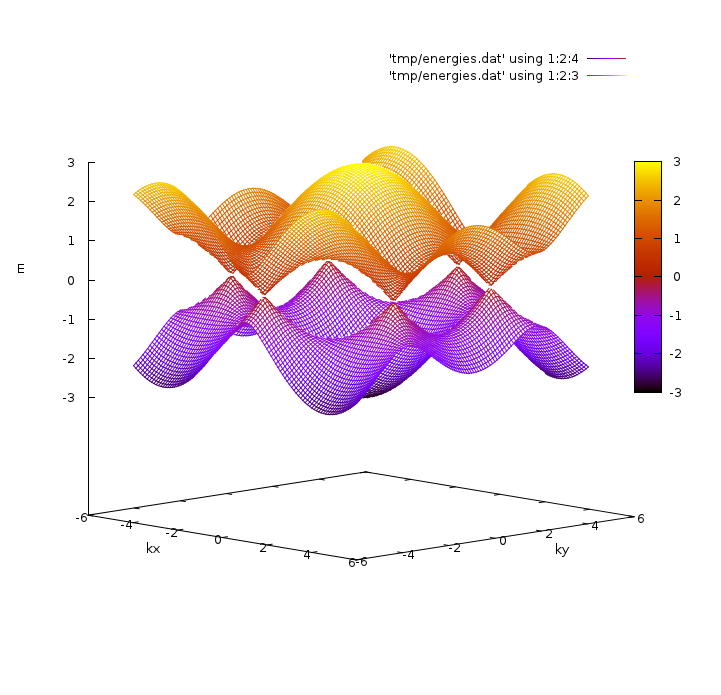
\includegraphics[width=0.5\textwidth]{energies-analytic-wireframe.png}
\caption{Energy levels of graphene. Energy (z axis) in units of eV.}
\label{fig:energies-analytic}
\end{figure}

In figure~\ref{fig:states-analytic}, I plotted the density of states for graphene (frequency distribution of energies) using the same tight binding model.

\begin{figure}[h!]
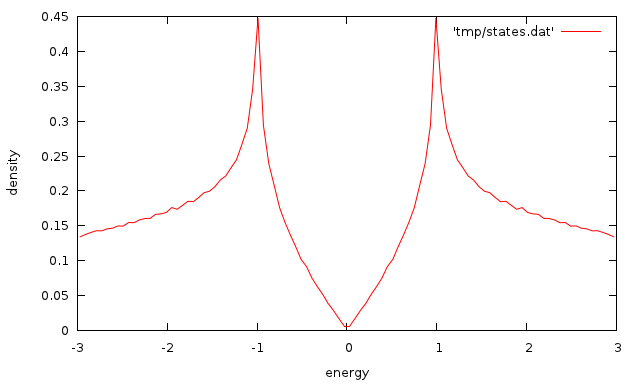
\includegraphics[width=0.5\textwidth]{states-analytic.png}
\caption{Density of states for graphene. Energy in units of eV.}
\label{fig:states-analytic}
\end{figure}

\section{Anderson model}

\subsection{Introduction}

The Anderson model~\cite{duxbury2011} consists of a Hamiltonian in the form of an adjacency matrix with random diagonal elements, which is solved for the energy levels (eigenvalues) and wave functions (eigenvectors).

Consider the graphene system shown in figure~\ref{fig:example-system}. The Hamiltonian for this system could, for example, be that of figure~\ref{fig:anderson-hamiltonian}. The diagonal elements are randomly uniformly selected from $(-W/2, W/2)$, where $W$ is the \emph{disorder width}. The $i$-$j$ element is 1 if sites $i$ and $j$ are neighbors and 0 otherwise.

\begin{figure}[h!]
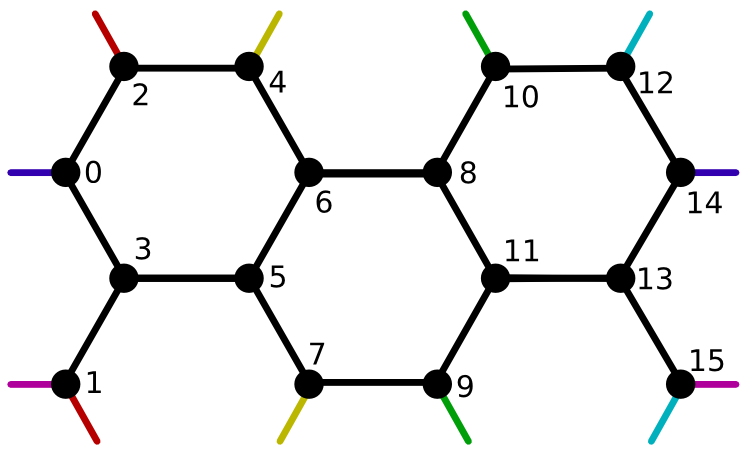
\includegraphics[width=0.5\textwidth]{example-system.png}
\caption{Example graphene system with 16 sites. Note: same-colored edges are connected via periodic boundary conditions.}
\label{fig:example-system}
\end{figure}

\begin{figure}[h!]
{\tiny \[ \left[
\begin{array}{cccccccccccccccc}
-.17 & 0 & 1 & 1 & 0 & 0 & 0 & 0 & 0 & 0 & 0 & 0 & 0 & 0 & 1 & 0 \\
0 & .47 & 1 & 1 & 0 & 0 & 0 & 0 & 0 & 0 & 0 & 0 & 0 & 0 & 0 & 1 \\
1 & 1 & -.44 & 0 & 1 & 0 & 0 & 0 & 0 & 0 & 0 & 0 & 0 & 0 & 0 & 0 \\
1 & 1 & 0 & -.12 & 0 & 1 & 0 & 0 & 0 & 0 & 0 & 0 & 0 & 0 & 0 & 0 \\
0 & 0 & 1 & 0 & -.03 & 0 & 1 & 1 & 0 & 0 & 0 & 0 & 0 & 0 & 0 & 0 \\
0 & 0 & 0 & 1 & 0 & .15 & 1 & 1 & 0 & 0 & 0 & 0 & 0 & 0 & 0 & 0 \\
0 & 0 & 0 & 0 & 1 & 1 & .36 & 0 & 1 & 0 & 0 & 0 & 0 & 0 & 0 & 0 \\
0 & 0 & 0 & 0 & 1 & 1 & 0 & .46 & 0 & 1 & 0 & 0 & 0 & 0 & 0 & 0 \\
0 & 0 & 0 & 0 & 0 & 0 & 1 & 0 & -.08 & 0 & 1 & 1 & 0 & 0 & 0 & 0 \\
0 & 0 & 0 & 0 & 0 & 0 & 0 & 1 & 0 & .17 & 1 & 1 & 0 & 0 & 0 & 0 \\
0 & 0 & 0 & 0 & 0 & 0 & 0 & 0 & 1 & 1 & .33 & 0 & 1 & 0 & 0 & 0 \\
0 & 0 & 0 & 0 & 0 & 0 & 0 & 0 & 1 & 1 & 0 & .41 & 0 & 1 & 0 & 0 \\
0 & 0 & 0 & 0 & 0 & 0 & 0 & 0 & 0 & 0 & 1 & 0 & -.49 & 0 & 1 & 1 \\
0 & 0 & 0 & 0 & 0 & 0 & 0 & 0 & 0 & 0 & 0 & 1 & 0 & -.48 & 1 & 1 \\
1 & 0 & 0 & 0 & 0 & 0 & 0 & 0 & 0 & 0 & 0 & 0 & 1 & 1 & -.38 & 0 \\
0 & 1 & 0 & 0 & 0 & 0 & 0 & 0 & 0 & 0 & 0 & 0 & 1 & 1 & 0 & .05
\end{array}
\right] \] }
\caption{Example Hamiltonian in the Anderson model.}
\label{fig:anderson-hamiltonian}
\end{figure}

\subsection{Density of states}

To find the energy levels $\varepsilon_i$, we need to solve for the eigenvalues $\varepsilon_i$ in the Schr\"{o}dinger equation $H \psi_i = \varepsilon_i \psi_i$, where $H$ is the Hamiltonian and the eigenvectors $\psi_i$ are the wave functions. I plotted two examples of this in figure~\ref{fig:anderson-states} (for two different disorder widths $W$).

\begin{figure}[h!]
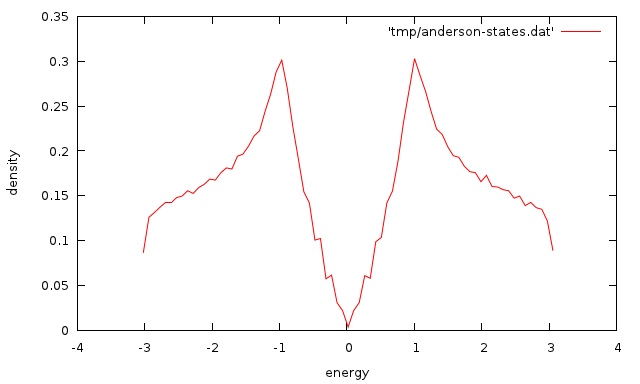
\includegraphics[width=0.4\textwidth]{anderson-states-W1.png}
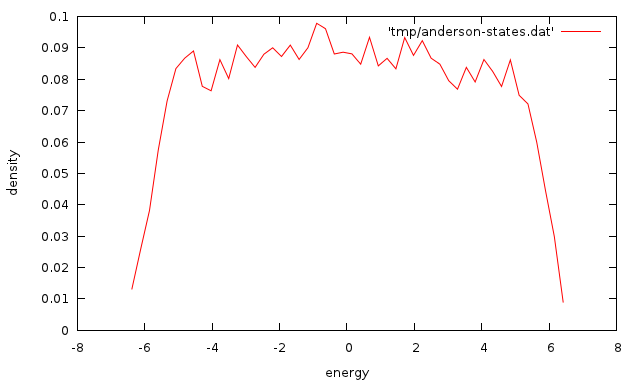
\includegraphics[width=0.4\textwidth]{anderson-states-W10.png}
\caption{Density of states using the Anderson model with disorder widths $W=1$ and $W=10$, respectively.}
\label{fig:anderson-states}
\end{figure}

The tight binding model and the Anderson model match fairly closely, as is evident by comparison of figures~\ref{fig:states-analytic} and \ref{fig:anderson-states}.

\subsection{Energy level spacing}

We can also find the spacing between subsequent energy levels $\varepsilon_i$ using this eigenvalue system. I plotted two examples of this in figure~\ref{fig:anderson-spacing}.

\begin{figure}[h!]
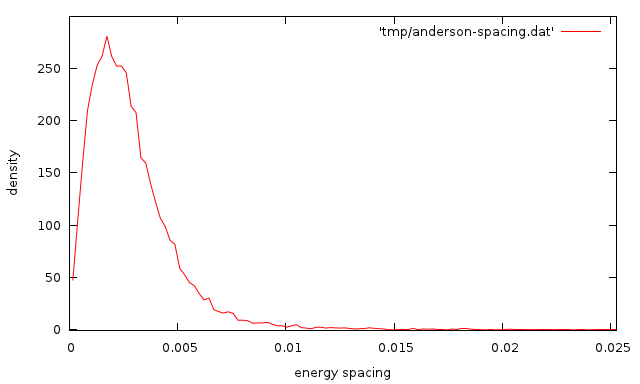
\includegraphics[width=0.4\textwidth]{anderson-spacing-W1.png}
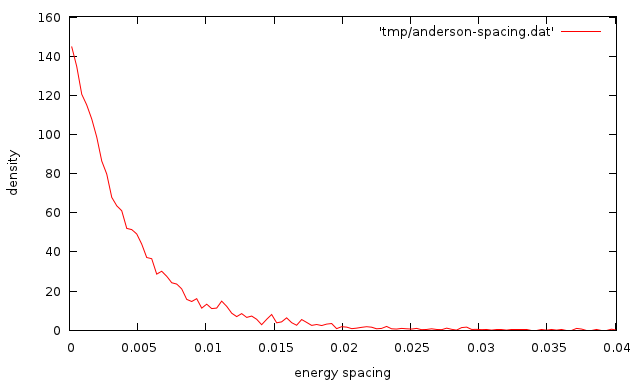
\includegraphics[width=0.4\textwidth]{anderson-spacing-W10.png}
\caption{Energy level spacing distribution using the Anderson model with disorder widths $W=1$ and $W=10$, respectively.}
\label{fig:anderson-spacing}
\end{figure}

\subsection{Inverse participation ratio}

Following \cite{kramer1993}, we can define an \emph{inverse participation ratio} (IPR) for each energy level $\varepsilon_i$ using the corresponding eigenvector $\psi_i$:

\[
\text{IPR} = \frac{\sum_j |\psi_i^{(j)}|^2}{n \sum_j |\psi_i^{(j)}|^4},
\]

where $n$ is the total number of sites in the system. Figure~\ref{fig:anderson-ipr} contains two plots plots of the IPR for a graphene system.

\begin{figure}[h!]
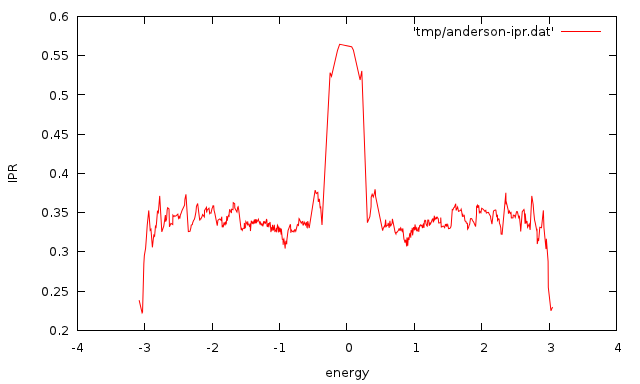
\includegraphics[width=0.4\textwidth]{anderson-ipr-W1.png}
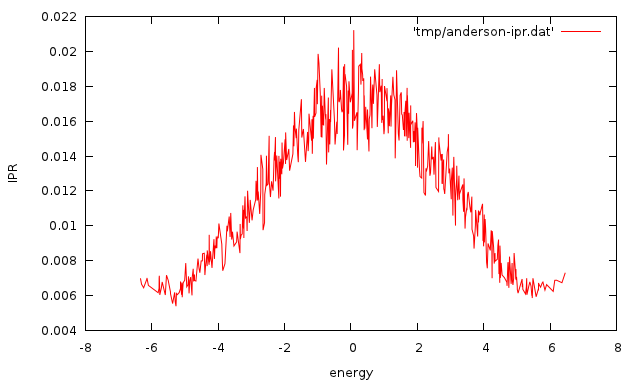
\includegraphics[width=0.4\textwidth]{anderson-ipr-W10.png}
\caption{Inverse participation ratio (IPR) with disorder widths $W=1$ and $W=10$, respectively.}
\label{fig:anderson-ipr}
\end{figure}


\begin{thebibliography}{9}

\bibitem{duxbury2011}
	P. Duxbury,
	\emph{PHY480: Project 3},
	\url{http://www.pa.msu.edu/~duxbury/courses/phy480/Project3_2011.pdf}
	(retrieved 2011-04-29).

\bibitem{kramer1993}
	B. Kramer and A. MacKinnon,
	\emph{Localization: theory and experiment},
	Reports on Progress in Physics 56, 1469 (1993).

\bibitem{reich2002}
	S. Reich, J. Maultzsch, and C. Thomsen,
	\emph{Tight-binding description of graphene},
	Phys. Rev. B66, 035412 (2002).

\end{thebibliography}

\end{document}
